\documentclass[addpoints,ngerman,12pt,answers]{exam}
\usepackage{babel}
\usepackage[top=2cm,bottom=2.5cm,left=1.5cm,right=1.5cm]{geometry}
\usepackage[utf8]{inputenc}
\usepackage[T1]{fontenc}
\usepackage{booktabs}
\usepackage{graphicx}
\usepackage{csquotes}
\usepackage{paralist}
%\usepackage{wasysym}
%\usepackage[math]{iwona}
\usepackage{setspace}
\usepackage{amsmath} 
\usepackage[math]{iwona}
\usepackage{setspace}
\usepackage{enumitem}
\usepackage{amsmath}
\usepackage{amsfonts}


\pointpoints{Point}{Points}
\bonuspointpoints{Bonuspunkt}{Bonuspunkte}
\renewcommand{\solutiontitle}{\noindent\textbf{Solution:}\enspace}

\chqword{Frage}   
\chpgword{Seite} 
\chpword{Punkte}   
\chbpword{Bonus Points} 
\chsword{Erreicht}   
\chtword{Gesamt}

\checkboxchar{\Square}
\checkedchar{\CheckedBox}

\pagestyle{headandfoot}
\runningheadrule
\firstpageheader{ECO202}{Week W5-6}{}
\runningheader{ECO202}{Week W5-6}{}
\firstpagefooter{ECO202}{Week W5-6}{\thepage\,/\,\numpages}
\runningfooter{ECO202}{Week W5-6}{\thepage\,/\,\numpages}
\doublespacing

\begin{document}
	\vspace*{3em}
	
	\makebox[\textwidth]{Name:\enspace\hrulefill}
	
	\vspace*{3em}
	\begin{questions}
		\question The OPEC has decided to collectively lower the oil price, which will act as a one-time shock. Concurrently, expectations from households and firms have improved. These expectation shocks will persist until another exogenous change occurs. Assuming that the economy is initially in the steady state, answer the following questions using the AS/AD framework, specifying which parameters are changing.
		
		\begin{enumerate}[label=(\alph*)]
			\item Determine the \textit{initial} impact of OPEC's decision on inflation and the output gap. Draw a graph to illustrate it.
			\item Determine the \textit{overall} impact of OPEC's decision on inflation and the output gap.
			Draw a graph to illustrate it.
		\end{enumerate}
		\newpage
		\textbf{Solution}
		\begin{enumerate}[label=(\alph*)]
			\item The oil shock (i.e., a fall in $\bar{o}$) would lead to a rightward shift in the AS curve from AS1 to AS2. As household and firm's expectation improved, the consumption and investment would increase (i.e., $\bar{a}_C$ and $\bar{a}_I$) the AD curve would also shift right from AD1 to AD2. There would be an increase for the short-run output. However, the initial impact on the inflation would be ambiguous -- if AD move more than AS, it leads to a fall in inflation. Vice Versa. 
			\begin{figure}[htbp!]
				\centering
				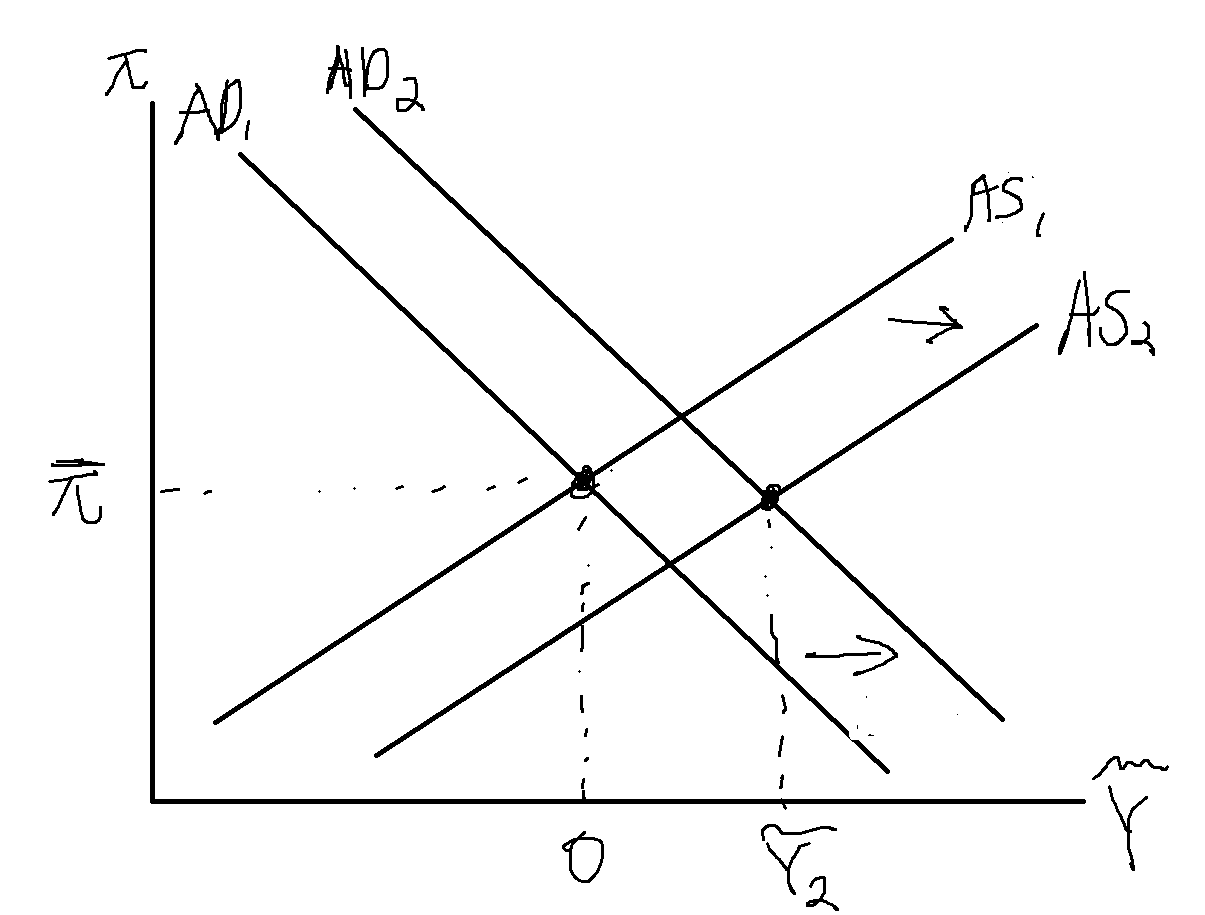
\includegraphics[width=0.5\linewidth]{Figure/q1a}
			\end{figure}
			
			
			\item After the initial impact, the $\bar{o}$ return to zero. Meanwhile, the $\bar{a}$ remain at the higher level. Recall the AS curve function:
			\[\pi_{t} = \pi_{t-1} +\bar{\nu} \widetilde{Y}_t + \bar{o}\]
			In period 3, the inflation rate would be equal to 
			\[\pi_3 = \pi_2 + \bar{\nu} \widetilde{Y}_3\]
			Since $\widetilde{Y}_3>0$, $\pi_3 >\pi_2$. The AS curve would gradually shift to the $AS_n$. 
			
			\begin{figure}[htbp!]
				\centering
				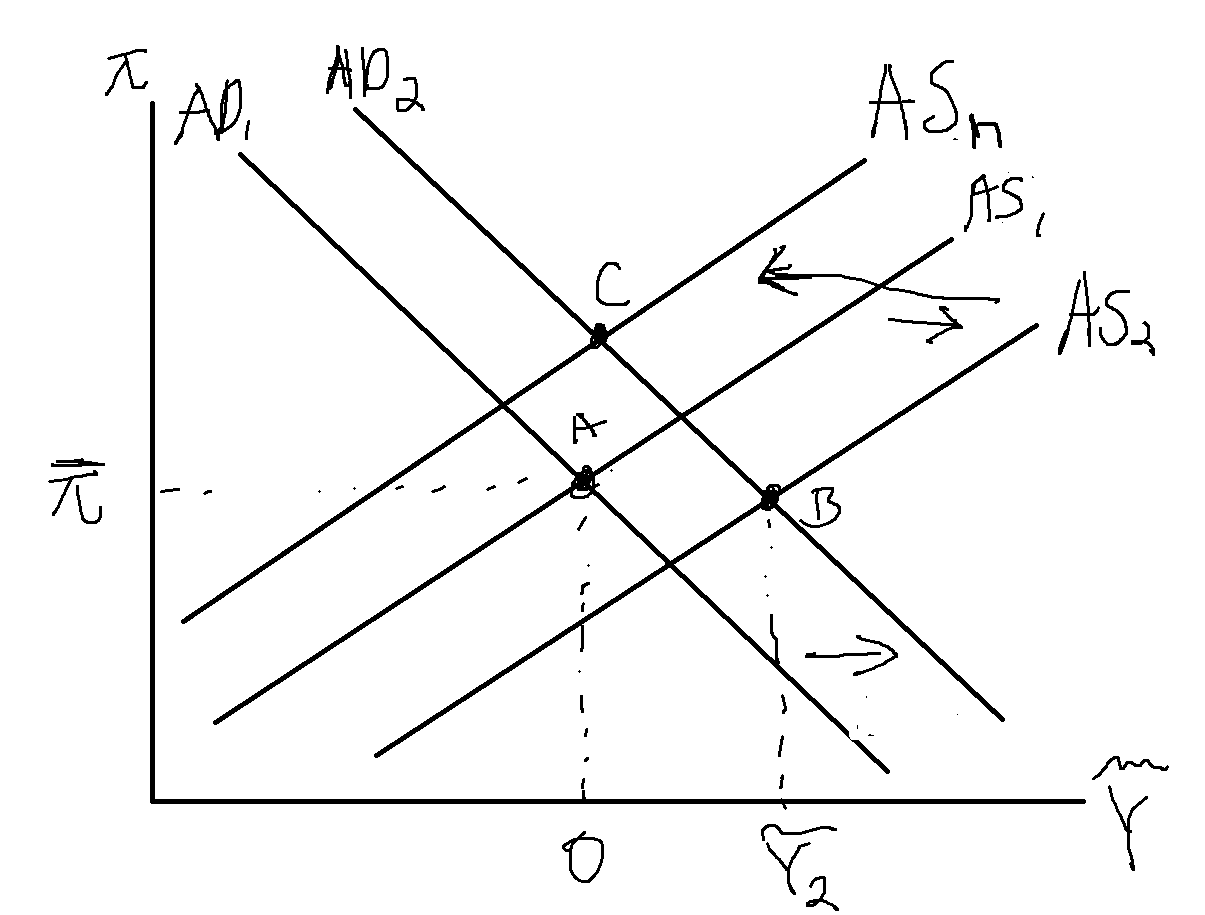
\includegraphics[width=0.5\linewidth]{Figure/q1b}
			\end{figure}

		\end{enumerate}
				
		
		
		\clearpage
		
		\question The figure below illustrates the perceived potential output as indicated by the policy marker in 1993, the actual potential output observed a couple of years later and the actual output.
		\begin{figure}[htbp!]
			\centering
			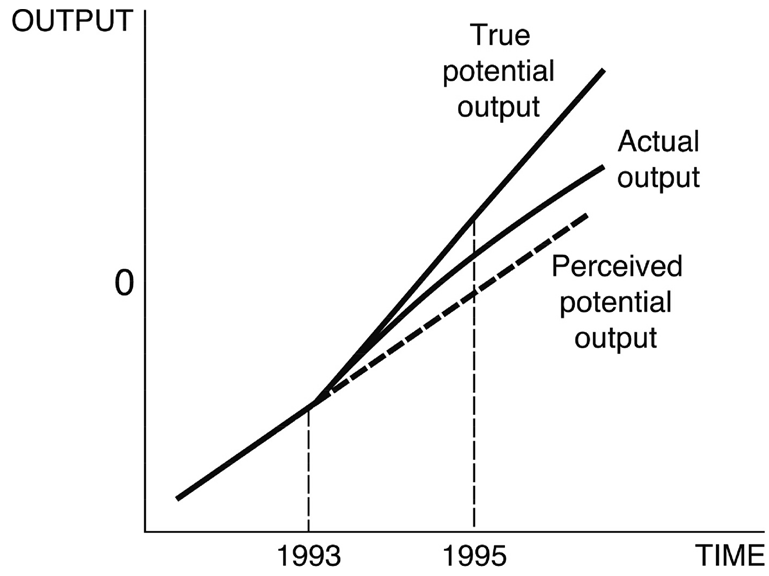
\includegraphics[width=0.5\linewidth]{Figure/q2}
		\end{figure}
		
		\begin{enumerate}[label=(\alph*)]
			\item What actions would the policymaker take based on the perceived potential output?
			\item What actions would the policymaker take based on the true potential output?
			\item If the policy is efficient, what should the actual output be like if the policymaker had the true potential output?
		\end{enumerate}
		\newpage
		\begin{solution}
			\begin{enumerate}[label=(\alph*)]
				\item Based on the perceived potential output, the policymaker would think that the economy is in an expansion. Therefore, it will raise the interest rate.
				\item Based on the true potential output, the policymaker would think that  the economy is in a recession. Therefore, it will lower the interest rate in order to stabilize the output.
				\item If the policymaker has lowered the interest rate, the actual output should be higher than it is. It is because lower the interest rate would lead to higher output based on the IS curve.
			\end{enumerate}
		\end{solution}		
		
	\end{questions}
	
%	\begin{center}
%		\combinedgradetable[h][questions]
%	\end{center}
	
\end{document}